\documentclass[11pt]{article}
\usepackage[margin=1in]{geometry}
\usepackage{amsmath,amssymb}
\usepackage{booktabs}
\usepackage{graphicx}
\usepackage{xcolor}
\usepackage{tikz}
\usetikzlibrary{arrows.meta,positioning,fit,calc,shapes.geometric}
\usepackage[numbers,sort&compress]{natbib}
\usepackage{float}
\usepackage{hyperref}
\usepackage[all]{hypcap}

\hypersetup{
  colorlinks=true,
  linkcolor=black,
  citecolor=black,
  urlcolor=blue
}

\title{Cinemath: Separating Pedagogical Reasoning from\\
Deterministic Educational Animation}
\author{Mauricio Tedeschi}
\date{\today}

\begin{document}
\maketitle

\begin{abstract}
Large language models can explain mathematical and physical reasoning, but
they are unreliable authors of low-level animation code. We present
\textsc{Cinemath}, an open-source pipeline that turns a typed or photographed
problem into a short educational Manim video while keeping those roles
strictly separated. A lightweight classifier routes each problem either to a
local catalog planner (SymPy-backed \texttt{plan\_*} functions that emit a
complete lesson plan without freeform generation) or to a freeform teacher
LLM that returns a structured plan of conceptual steps and named visual-tool
calls. Integration problems route to technique-specific catalog planners
(partial fractions, trigonometric substitution, $u$-substitution, integration
by parts, or elementary antiderivatives); stacked or SymPy-unwalkable integrals
fall through to freeform. Local compilers expand those calls into a validated animation script,
re-check freeform claims with SymPy (retrying on failure), and render with
Manim Community. Because scene construction never depends on free-form
model-generated Python, visual fidelity is controlled by hand-written
templates spanning paper arithmetic, algebra boards, calculus plots, formal
proofs, and quantum-field-theory diagrams including one-loop layouts and
renormalization-group flow sketches. We describe the architecture, the
classify-and-catalog layer, the plan schema, the visual-tool catalog, curated
and scraped problem banks, and a difficulty ladder from elementary arithmetic
through Peskin-style $\beta$-function problems.
\end{abstract}

\section{Introduction}

Educational animation systems such as Manim make it possible to present
equations, graphs, and diagrams with cinematic timing
\citep{manim2024community}. At the same time, frontier language models have
become competent tutors for multi-step mathematics and physics
\citep{anthropic2024claude}. Combining the two is attractive: given a
homework-style prompt, one would like a narrated visual solution rather than
a static wall of text.

A na\"ive approach---asking the model to emit Manim source directly---fails
in predictable ways. Generated code frequently invents nonexistent APIs,
breaks \LaTeX \ mid-expression, hard-codes fragile layout constants, or
silently skips pedagogically important beats. Even when the mathematics in
the explanation is correct, the animation layer may not compile.

\textsc{Cinemath} adopts the opposite contract. The language model never
authors Manim source. For common problem shapes it may not author the lesson
plan either: a classifier selects a local catalog planner that builds
\texttt{plan.json} with SymPy or exact arithmetic. Only when no planner fits
does a freeform teacher return a versioned JSON plan---normalized statement,
final answer, conceptual steps, and a non-empty list of visual tools from a
fixed catalog. All animation construction, validation, and rendering remain
local and deterministic. This separation mirrors classical compiler design:
the front end emits an intermediate representation; trusted backends lower it
to pixels.

The system is deliberately domain-agnostic at the plan level. Instead of a
single mutually exclusive ``problem type,'' the plan selects a composition of
tools (for example, a rectangular double integral may request a region
outline, an equation board, a three-dimensional surface, and a final answer
beat). Specialized QFT tools cover interaction Lagrangians, tree-level
$1\to 2$ decays, one-loop / 1PI diagrams, and two-dimensional
renormalization-group flow fields of the kind appearing in textbook exercises
\citep{peskin1995introduction}.

\section{Architecture}

Figure~\ref{fig:pipeline} summarizes the end-to-end pipeline. A run begins
with a text file, Markdown note, or image of a problem. Images are OCR'd /
transcribed; the extracted statement is then classified. Classification calls
exactly one tool: either a catalog \texttt{plan\_*} entry (quadratic, linear
systems, derivatives, technique-specific integrals---partial fractions,
trigonometric substitution, $u$-substitution, integration by parts, elementary
definite / improper integrals---partial derivatives, double / triple box
integrals, paper arithmetic, \ldots) or \texttt{teach\_freeform}. Catalog
planners emit a complete plan locally. When a catalog planner cannot finish
an integral (for example a stacked $\sqrt{\tan x}$ exercise), it signals
freeform rather than silently stacking techniques inside one lesson. The
freeform teacher may call local arithmetic tools for long multiplication,
division, addition, or subtraction so that digit-level results are
ground-truth rather than model-invented; its plan is then verified with SymPy
and retried with structured feedback on failure. Local template compilers
expand \texttt{visuals[]} into an internal animation DSL, prepend a
problem-statement scene, and validate the script. Manim finally renders
\texttt{animation.mp4} together with a Markdown lesson transcript.

\begin{figure}[H]
\centering
\resizebox{\textwidth}{!}{%
\begin{tikzpicture}[
  font=\sffamily\small,
  >=Latex,
  node distance=0.45cm and 0.38cm,
  stage/.style={
    draw=black!65,
    rounded corners=2.5pt,
    align=center,
    inner xsep=5pt,
    inner ysep=4pt,
    minimum height=0.95cm,
    minimum width=2.15cm,
    fill=black!4
  },
  llm/.style={stage, fill=blue!10},
  local/.style={stage, fill=green!10},
  file/.style={
    draw=black!50,
    dashed,
    rounded corners=1.5pt,
    align=center,
    inner sep=3pt,
    font=\ttfamily\scriptsize,
    fill=white
  },
  arr/.style={->, thick, black!65}
]
  % Top row
  \node[stage] (in) {Input\\[-0.1em]{\scriptsize text / image}};
  \node[llm, right=of in] (extract) {Extract\\[-0.1em]{\scriptsize statement}};
  \node[llm, right=of extract] (classify) {Classify\\[-0.1em]{\scriptsize plan\_* / freeform}};
  \node[local, right=of classify] (catalog) {Catalog\\[-0.1em]{\scriptsize plan\_* + SymPy}};
  \node[llm, below=0.55cm of catalog] (teach) {Freeform teach\\[-0.1em]{\scriptsize + arith tools}};

  \draw[arr] (in) -- (extract);
  \draw[arr] (extract) -- (classify);
  \draw[arr] (classify) -- (catalog);
  \draw[arr] (classify) |- (teach);

  % Bridge artifact
  \node[file, below=0.55cm of teach] (plan) {plan.json};
  \draw[arr] (catalog) -- (plan);
  \draw[arr] (teach) -- (plan);

  % Bottom row
  \node[local, below=0.55cm of plan] (verify) {Verify\\[-0.1em]{\scriptsize freeform only}};
  \node[local, right=of verify] (compile) {Compile\\[-0.1em]{\scriptsize visual tools}};
  \node[local, right=of compile] (validate) {Validate\\[-0.1em]{\scriptsize animation DSL}};
  \node[local, right=of validate] (render) {Render\\[-0.1em]{\scriptsize Manim}};

  \draw[arr] (plan) -- (verify);
  \draw[arr] (verify) -- (compile);
  \draw[arr] (compile) -- (validate);
  \draw[arr] (validate) -- (render);

  \node[file, below=0.4cm of verify] (ver) {verify.json};
  \node[file, below=0.4cm of compile] (anim) {animation.json};
  \node[file, below=0.4cm of render] (mp4) {animation.mp4};
  \draw[arr] (verify) -- (ver);
  \draw[arr] (compile) -- (anim);
  \draw[arr] (render) -- (mp4);

  \node[anchor=south west, font=\scriptsize, text=black!60]
    at ([yshift=0.4cm]in.north west) {%
    {\tikz[baseline=-0.45ex]\fill[blue!10,draw=black!65,rounded corners=1pt]
      (0,0) rectangle (0.4,0.2);}~~LLM
    \quad
    {\tikz[baseline=-0.45ex]\fill[green!10,draw=black!65,rounded corners=1pt]
      (0,0) rectangle (0.4,0.2);}~~local
  };
\end{tikzpicture}%
}
\caption{Cinemath pipeline. Blue stages may call the language model; green stages
are fully local. Classification routes to a local catalog planner or a freeform
teacher. \texttt{verify.json} is written for freeform plans (with SymPy retry);
catalog plans skip that stage. Neither path authors Manim scenes.}
\label{fig:pipeline}
\end{figure}

\subsection{Trust boundary}

The critical invariant is that \texttt{animation.json} is never authored by
the model. Catalog planners fill typed visual fields locally; the freeform
teacher may choose \emph{which} visual capabilities to invoke and fill their
typed fields (coefficients, region bounds, Feynman labels, $\beta$-function
expressions). Scene graph construction, caption timing, equation-chain
morphs, and camera moves live in versioned Python modules under
\texttt{templates/} and \texttt{render\_engine/}.

\subsection{Artifacts}

Each successful \texttt{cinemath solve} run creates a timestamped directory
containing
\begin{itemize}
  \item \texttt{problem.txt} --- normalized statement with ASCII \LaTeX\ in
    \texttt{\$...\$};
  \item \texttt{plan.json} --- lesson plan (version~2), from a catalog planner
    or the freeform teacher;
  \item \texttt{verify.json} --- freeform SymPy check / retry summary (omitted
    for catalog plans);
  \item \texttt{lesson.md} --- human-readable lesson transcript;
  \item \texttt{animation.json} --- validated internal DSL;
  \item \texttt{animation.mp4} --- rendered video (optional retained
    \texttt{media/} with \texttt{--keep-media}).
\end{itemize}

\subsection{Catalog planners}
\label{sec:catalog}

When classification hits a catalog entry, a local \texttt{plan\_*} function in
\texttt{src/cinemath/planners/} builds the entire plan---steps, answer, and
\texttt{visuals[]}---using SymPy or exact arithmetic. Shipped planners include
\texttt{plan\_quadratic}, \texttt{plan\_linear}, \texttt{plan\_linear\_system\_2d/3d},
\texttt{plan\_percent\_off}, \texttt{plan\_derivative},
\texttt{plan\_partial\_fractions}, \texttt{plan\_trig\_substitution},
\texttt{plan\_u\_substitution}, \texttt{plan\_integration\_by\_parts},
\texttt{plan\_definite\_integral} (elementary antiderivatives and improper
limits only), \texttt{plan\_partial\_derivative},
\texttt{plan\_double\_integral}, \texttt{plan\_triple\_integral}, and the four
\texttt{plan\_long\_*} arithmetic planners. The classifier picks exactly one
integration technique; \texttt{plan\_definite\_integral} rejects integrands
that need a specialized planner, and unwalkable stacked integrals route to
\texttt{teach\_freeform}. Proofs, series arguments, vector calculus, and QFT
exercises also fall through to \texttt{teach\_freeform}.

\subsection{Worked example: quadratic roots}
\label{sec:worked}

Figure~\ref{fig:artifact-shapes} summarizes the on-disk contract for a real run of
\texttt{examples/04\_quadratic.txt} ($x^{2}-5x+6=0$; also
\texttt{problems/curated/04\_quadratic.txt}).
Classification selects \texttt{plan\_quadratic}, so the LLM does not write
\texttt{plan.json}; local stages emit \texttt{animation.json}, then Manim
produces \texttt{animation.mp4}. The JSON chips show \emph{shape}, not full
payloads. Figure~\ref{fig:artifact-frames} shows four frames from that same
video.

\begin{figure}[H]
\centering
\begin{tikzpicture}[
  font=\sffamily\scriptsize,
  >=Latex,
  box/.style={
    draw=black!50, rounded corners=2.5pt,
    align=center, inner xsep=3pt, inner ysep=5pt,
    minimum width=2.55cm, minimum height=2.5cm,
    fill=black!2
  },
  llm/.style={box, fill=blue!6, draw=blue!35!black!55},
  loc/.style={box, fill=green!6, draw=green!35!black!55},
  arr/.style={->, thick, black!55}
]
  \node[box] (c1) {%
    {\ttfamily\bfseries\tiny input}\\[4pt]
    {\sffamily\footnotesize text / image}\\[3pt]
    {\ttfamily\tiny Solve}\\[-1pt]
    {\ttfamily\tiny $x^{2}-5x+6=0$}
  };
  \node[llm, right=0.42cm of c1] (c2) {%
    {\color{blue!50!black}\ttfamily\bfseries\tiny classify}\\[4pt]
    {\ttfamily\tiny plan\_quadratic}\\[3pt]
    {\sffamily\tiny (not freeform)}
  };
  \node[loc, right=0.42cm of c2] (c3) {%
    {\color{green!35!black}\ttfamily\bfseries\tiny plan.json}\\[4pt]
    {\ttfamily\tiny version}\\[-1pt]
    {\ttfamily\tiny steps[\,]}\\[-1pt]
    {\ttfamily\tiny visuals[\,]}\\[3pt]
    {\sffamily\tiny plot\_2d $\cdot$ board $\cdot$ answer}
  };
  \node[loc, right=0.42cm of c3] (c4) {%
    {\color{green!35!black}\ttfamily\bfseries\tiny animation.json}\\[4pt]
    {\ttfamily\tiny scenes[\,]}\\[-1pt]
    {\ttfamily\tiny objects[\,]}\\[-1pt]
    {\ttfamily\tiny actions[\,]}
  };
  \node[loc, right=0.42cm of c4] (c5) {%
    {\color{green!35!black}\ttfamily\bfseries\tiny animation.mp4}\\[4pt]
    {\sffamily\footnotesize video}\\[3pt]
    {\ttfamily\tiny problem $\to$ plot}\\[-1pt]
    {\ttfamily\tiny $\to$ board $\to$ answer}
  };

  \foreach \a/\b in {c1/c2, c2/c3, c3/c4, c4/c5}
    \draw[arr] (\a) -- (\b);

  \node[font=\scriptsize, text=black!60, anchor=north]
    at ([yshift=-0.22cm]current bounding box.south) {%
    {\tikz[baseline=-0.45ex]\fill[blue!6,draw=blue!35!black!55,rounded corners=1pt]
      (0,0) rectangle (0.4,0.2);}~~LLM stage
    \quad
    {\tikz[baseline=-0.45ex]\fill[green!6,draw=green!35!black!55,rounded corners=1pt]
      (0,0) rectangle (0.4,0.2);}~~local artifact%
    };
\end{tikzpicture}
\caption{Quadratic catalog run as pictographs. Classification selects
\texttt{plan\_quadratic}; the plan and animation artifacts are local.
Boxes sketch \emph{shape}, not complete file contents.}
\label{fig:artifact-shapes}
\end{figure}

\begin{figure}[H]
\centering
\begin{minipage}[t]{0.48\textwidth}
\centering
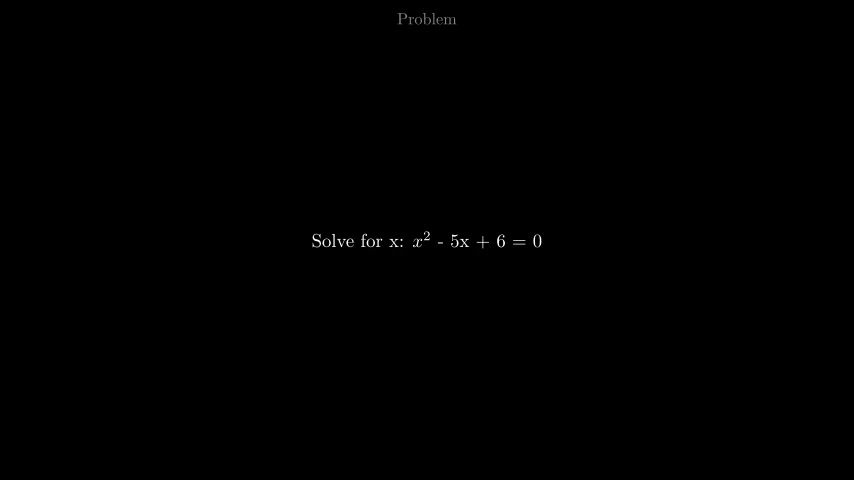
\includegraphics[width=\linewidth]{figures/ex_problem.jpg}\\[2pt]
{\footnotesize (a) Problem beat}
\end{minipage}\hfill
\begin{minipage}[t]{0.48\textwidth}
\centering
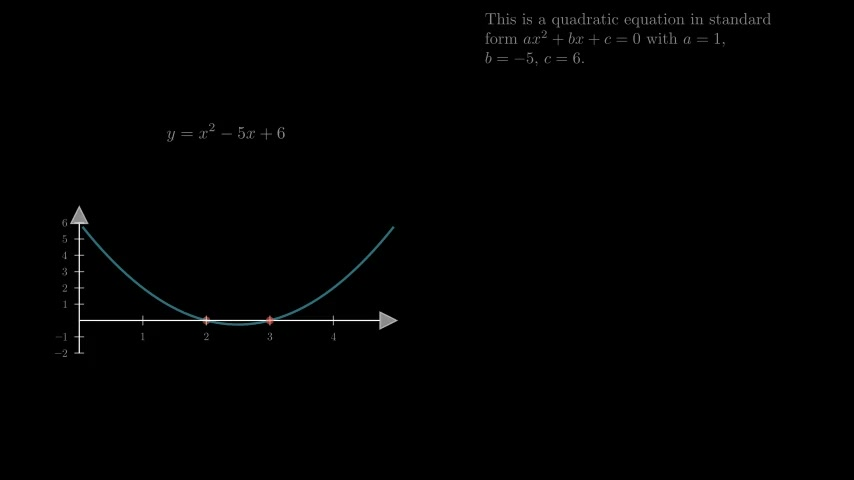
\includegraphics[width=\linewidth]{figures/ex_plot.jpg}\\[2pt]
{\footnotesize (b) \texttt{plot\_2d} beat}
\end{minipage}

\vspace{0.35em}
\begin{minipage}[t]{0.48\textwidth}
\centering
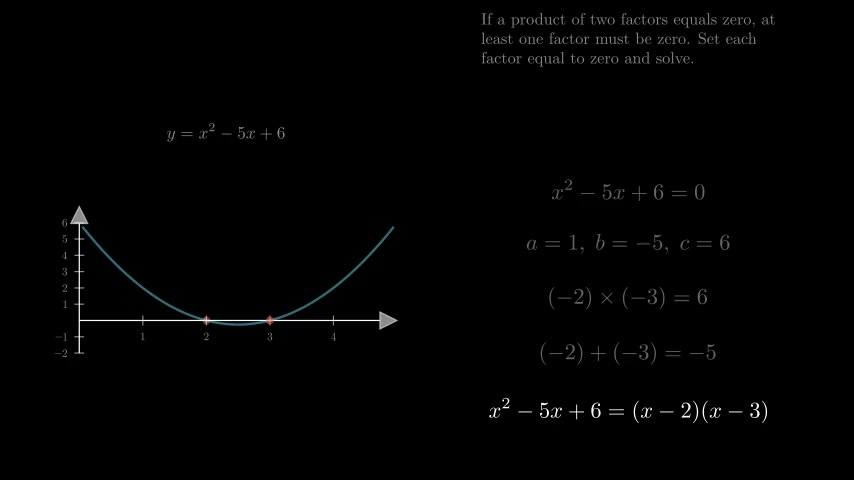
\includegraphics[width=\linewidth]{figures/ex_board.jpg}\\[2pt]
{\footnotesize (c) Equation board}
\end{minipage}\hfill
\begin{minipage}[t]{0.48\textwidth}
\centering
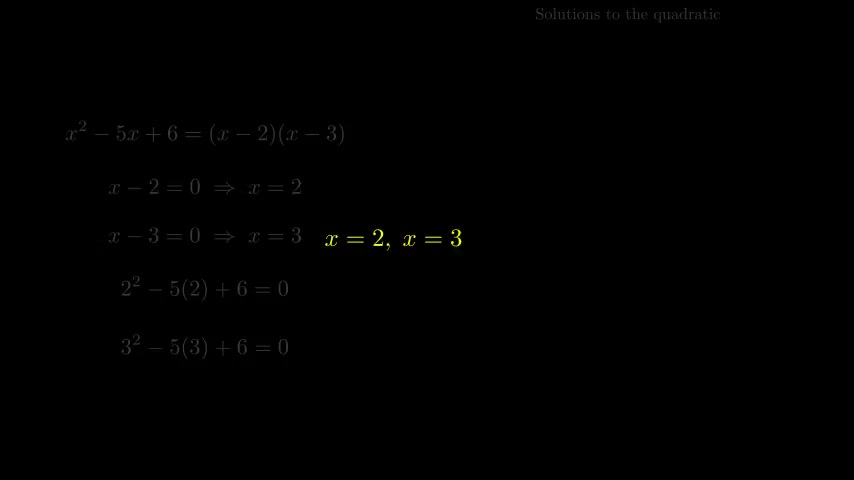
\includegraphics[width=\linewidth]{figures/ex_answer.jpg}\\[2pt]
{\footnotesize (d) Answer beat}
\end{minipage}
\caption{Frames from the same quadratic \texttt{animation.mp4}, in order.}
\label{fig:artifact-frames}
\end{figure}

\section{Teacher plan schema}

Plans are JSON objects with schema version~2. The required fields are
\texttt{problem}, \texttt{answer}, \texttt{steps}, and a non-empty
\texttt{visuals} array. Each step carries a short board title, a one-to-three
sentence explanation, and zero or more display-math fragments. Visual entries
are tagged by \texttt{tool} and validated against a closed catalog
(Section~\ref{sec:tools}). Catalog planners and the freeform teacher share this
schema so the compilers need not know which front end produced the plan.

The freeform system prompt forbids animation design language: the model must
not mention Manim, colors, camera angles, or frame timing. Mathematical hygiene
rules require ASCII \LaTeX \ (no Unicode glyphs such as $\mu$ or $\phi$ written
as code points) and consistent dollar wrapping in prose fields. Pure formula
fields omit surrounding dollars so that Manim's \texttt{MathTex} path remains
unambiguous.

For long arithmetic outside the catalog path, the freeform teacher must call
the matching local tool (\texttt{long\_multiply}, \texttt{long\_divide},
\texttt{long\_add}, or \texttt{long\_subtract}) and copy the returned digits
into both \texttt{answer} and the corresponding \texttt{paper\_long\_*} visual.
Catalog arithmetic planners skip that round-trip and write the digits
directly.

\section{Visual tools}
\label{sec:tools}

Table~\ref{tab:tools} lists the current catalog. Tools are intentionally
composable: a proof uses \texttt{state\_claim}, \texttt{equation\_board}, and
\texttt{show\_qed}; a rectangular double integral typically stacks region,
board, surface, and answer beats; a Yukawa $\beta$-function exercise may
combine a Lagrangian frame, one or more loop diagrams, the equation board,
an RG flow field, and a highlighted answer.

\begin{table}[H]
\centering
\caption{Visual-tool catalog exposed to the teacher (plan version~2).}
\label{tab:tools}
\begin{tabular}{@{}ll@{}}
\toprule
Tool & Role \\
\midrule
\texttt{equation\_board} & Caption + stacked derivation lines \\
\texttt{state\_claim} / \texttt{show\_qed} & Proof opener / closer \\
\texttt{plot\_2d} & Quadratic parabola with marked roots \\
\texttt{plot\_integral\_1d} & Shaded definite integral under a curve \\
\texttt{show\_region\_rectangle} & 2D rectangular integration region \\
\texttt{plot\_surface\_3d} & Surface over a rectangular domain \\
\texttt{paper\_long\_*} & Stacked paper arithmetic layouts \\
\texttt{show\_lagrangian} & Interaction / Lagrangian setup \\
\texttt{feynman\_1to2} & Tree-level $1\to 2$ decay diagram \\
\texttt{feynman\_loop} & One-loop layouts (bubble, 4-point, Yukawa triangle) \\
\texttt{rg\_flow\_2d} & Arrow field from $\beta_x(x,y)$, $\beta_y(x,y)$ \\
\texttt{show\_answer} & Final highlighted answer beat \\
\bottomrule
\end{tabular}
\end{table}

Each tool maps to a small compiler that emits objects in an internal DSL
(\texttt{math}, \texttt{prose}, \texttt{axes}, \texttt{plot}, \texttt{feynman},
\texttt{flow\_field}, \ldots) and a short action list
(\texttt{write}, \texttt{create}, \texttt{indicate}, \texttt{wait}, \ldots).
The renderer interprets that DSL only after schema validation, including
safe-expression checks for plots and RG fields.

\section{Rendering and pedagogy}

Algebraic derivations use an equation chain: the previous line is dimmed,
the board scrolls to make room, and a copy morphs into the next expression
via Manim's \texttt{TransformMatchingTex}. Step explanations become wrapped
instruction banners sized for full-frame or split-stage layouts. Every video
opens with a problem-statement beat so the viewer sees the claim before the
solution choreography begins.

Two- and three-dimensional graph helpers auto-select axis ranges, optionally
shade regions, and keep captions clear of plot chrome. QFT helpers draw
schematic Feynman layouts and sample renormalization-group arrow fields from
safe arithmetic expressions in variables $(x,y)$, which the teacher uses as
stand-ins for couplings such as $(\lambda,g)$.

\section{Examples and problem banks}

The repository ships a curated difficulty ladder under
\texttt{problems/curated/} (symlinked as \texttt{examples/} at the repo root),
from elementary word problems through linear systems, Calc~II/III catalog
targets, tree-level scalar decay, and related QFT exercises
(Table~\ref{tab:ladder}). Scraped banks from Paul's Online Math Notes (Lamar),
MIT~18.01/18.02, Arizona Math~129, and OpenStax live under \texttt{problems/}
with per-topic \texttt{meta.json} manifests; sync with
\texttt{scripts/sync\_problem\_banks.py}. In practice the same architecture
also covers photographed textbook problems, including Callan--Symanzik
$\beta$-function computations in pseudoscalar Yukawa theory with qualitative
RG-flow sketches \citep{peskin1995introduction}.
Figure~\ref{fig:snapshots} shows representative frames from rendered lessons
across several tool recipes.

\begin{figure}[H]
\centering
\setlength{\tabcolsep}{4pt}
\renewcommand{\arraystretch}{0.85}
\begin{tabular}{@{}c@{\hspace{0.28cm}}c@{}}
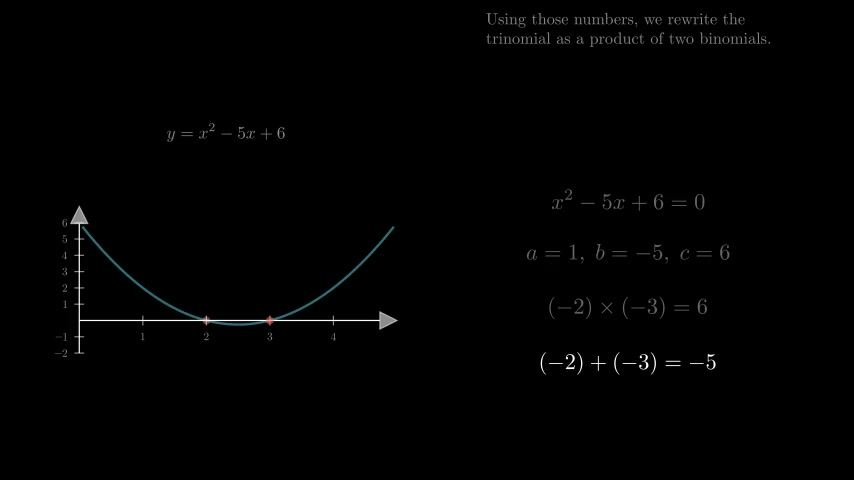
\includegraphics[width=0.40\textwidth]{figures/snap_quadratic.jpg} &
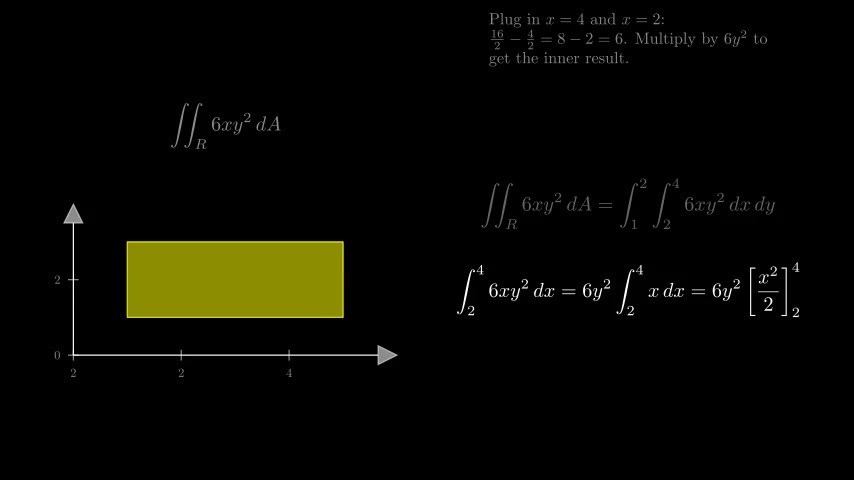
\includegraphics[width=0.40\textwidth]{figures/snap_integral.jpg} \\
{\footnotesize (a) Quadratic + \texttt{plot\_2d}} &
{\footnotesize (b) Double-integral region} \\[0.35em]
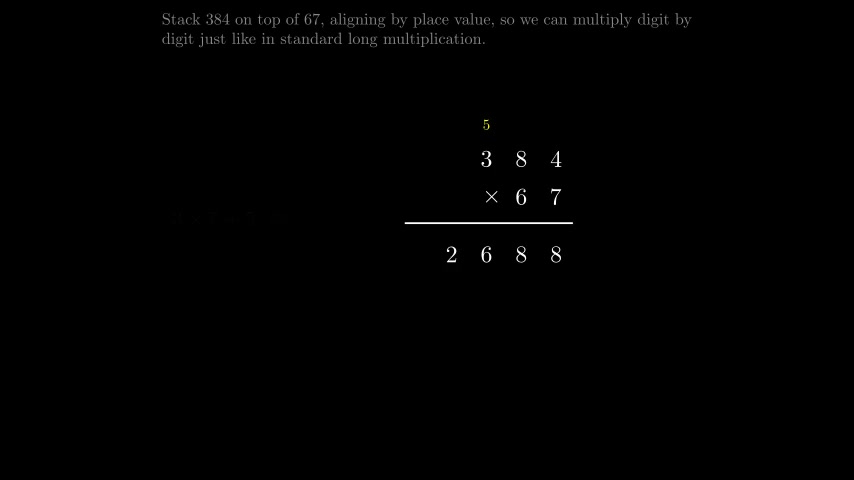
\includegraphics[width=0.40\textwidth]{figures/snap_multiply.jpg} &
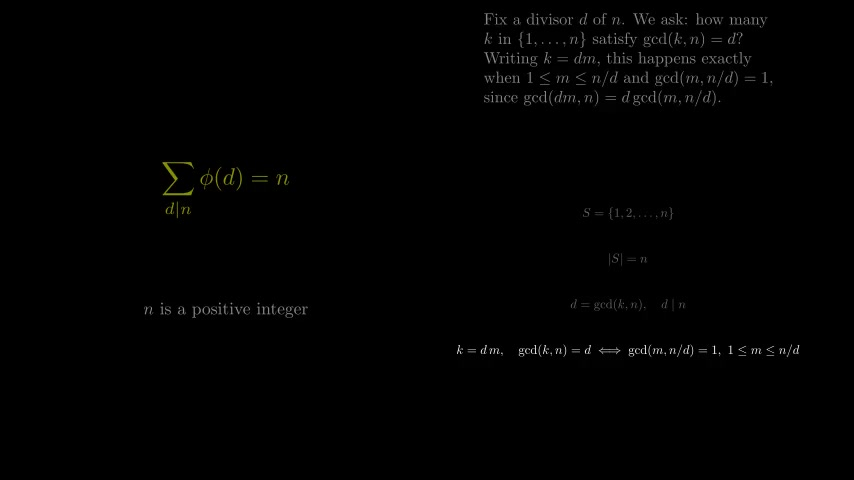
\includegraphics[width=0.40\textwidth]{figures/snap_proof.jpg} \\
{\footnotesize (c) Paper long multiplication} &
{\footnotesize (d) Totient proof board} \\[0.35em]
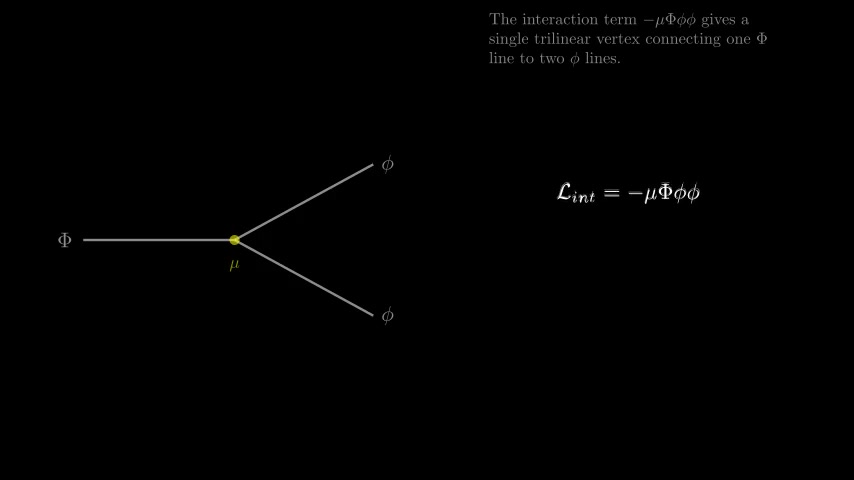
\includegraphics[width=0.40\textwidth]{figures/snap_decay.jpg} &
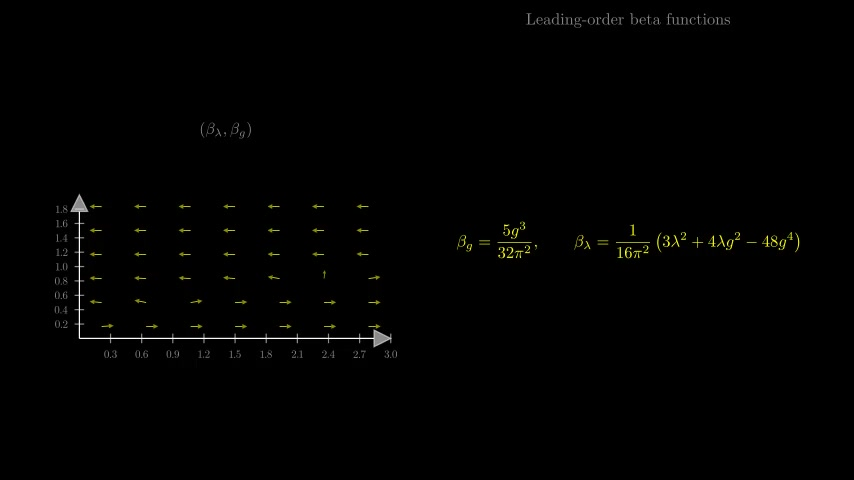
\includegraphics[width=0.40\textwidth]{figures/snap_rg.jpg} \\
{\footnotesize (e) Tree-level $1\to 2$ decay} &
{\footnotesize (f) RG flow + one-loop betas}
\end{tabular}
\caption{Representative frames from \textsc{Cinemath} lessons (algebra through QFT).}
\label{fig:snapshots}
\end{figure}

\begin{table}[H]
\centering
\caption{Representative curated ladder (\texttt{problems/curated/}).}
\label{tab:ladder}
\begin{tabular}{@{}clll@{}}
\toprule
Level & Example & Planner & Typical visuals \\
\midrule
1--3 & Arithmetic / percent & catalog / freeform & \texttt{equation\_board} \\
4 & Quadratic & \texttt{plan\_quadratic} & \texttt{plot\_2d}, board, answer \\
6--7 & Derivative / double integral & catalog & board / region+surface \\
8 & Euler totient identity & freeform & claim, board, QED \\
9--10 & Improper integral / $\Phi\to\phi\phi$ & catalog / freeform & board / Feynman \\
11--15 & Paper long arithmetic & \texttt{plan\_long\_*} & \texttt{paper\_long\_*} \\
16--17 & Linear systems $2\times2$ / $3\times3$ & catalog & board, answer \\
18--21 & IBP / sine / partial / triple & catalog & board (+ plot/region) \\
\bottomrule
\end{tabular}
\end{table}

\section{Discussion}

Restricting generation to a typed intermediate representation---and, for
catalog hits, removing freeform plan authorship entirely---trades expressive
freedom for reliability. New visual genres and new \texttt{plan\_*} entries
require local code, but once written they are reused across every problem that
routes to them. Classification already implements a coarse gate: only the
chosen planner's parameters (or the freeform teach path) are in play, which
keeps context smaller as the planner registry grows. Visual tools remain tagged
by domain (\texttt{core}, \texttt{proof}, \texttt{calculus},
\texttt{arithmetic}, \texttt{qft}) for further prompt gating if needed.

Limitations remain. Verification coverage is uneven across freeform tools;
symbolic checks are strongest for arithmetic and selected algebraic payloads.
Catalog calculus planners now cover partial fractions, trigonometric
substitution, $u$-substitution, integration by parts, and elementary definite
integrals with stepped SymPy \texttt{manualintegrate} walks; stacked or
SymPy-unwalkable integrals defer to the freeform teacher rather than
auto-chaining techniques inside one catalog lesson. Remaining gaps include
series tests, vector calculus, and richer diagrammatic calculus. Pedagogical
quality on the freeform path still depends on the teacher's step
decomposition. Schematic Feynman diagrams are illustrative rather than
automated 1PI generators, and RG flow fields visualize provided $\beta$
expressions rather than deriving them. Finally, image OCR inherits the usual
transcription failure modes for dense blackboard photography.

Natural extensions include richer series and vector-calculus planners,
tighter SymPy verification of board lines, golden tests over the curated
ladder and Lamar banks organized by \texttt{plan\_*}, and optional narration
audio aligned to scene captions.

\section{Conclusions}

\textsc{Cinemath} demonstrates a practical split between LLM routing /
pedagogy and deterministic educational animation. Classification and catalog
planners keep common problems off the freeform path; when the teacher is
needed, it still never writes animation code. Local visual tools compile and
Manim renders. The resulting pipeline produces short lesson videos across
arithmetic, algebra, calculus, proof, and selected quantum field theory
topics, backed by curated examples and scraped Calc~II/III problem banks.
Source code and examples are available in the accompanying repository.

\section*{Software}

Implementation is in Python~3.12+ using the Anthropic API
\citep{anthropic2024claude}, SymPy \citep{meurer2017sympy}, Typer, and Manim
Community \citep{manim2024community}. Optional model overrides separate a
fast classify/OCR model from the freeform teach model. The command-line
entrypoint is
\begin{verbatim}
uv run cinemath solve path/to/problem
\end{verbatim}
Artifacts for each run are written under \texttt{outputs/}.

\appendix

\section{Reproducibility}
\label{app:repro}

From the project root,
\begin{verbatim}
uv sync
cp .env.example .env   # set ANTHROPIC_API_KEY
uv run cinemath solve examples/04_quadratic.txt
uv run cinemath solve problems/curated/18_lamar_integration_by_parts.txt
uv run cinemath solve problems/by-type/plan_trig_substitution/lamar-calc-ii-trig-substitutions/prob-01.txt
uv run python scripts/sync_problem_banks.py   # refresh scraped banks
\end{verbatim}

\bibliographystyle{unsrtnat}
\bibliography{references}

\end{document}
